
\paragraph{Fonctionnement}

Cette partie va illustrer ce rapport d'un jeux de copies d'�crans
retracant les fonctionnalit�s implant�s.


1 Cr�ation du graphe

\begin{figure}[ht]
  \centering
  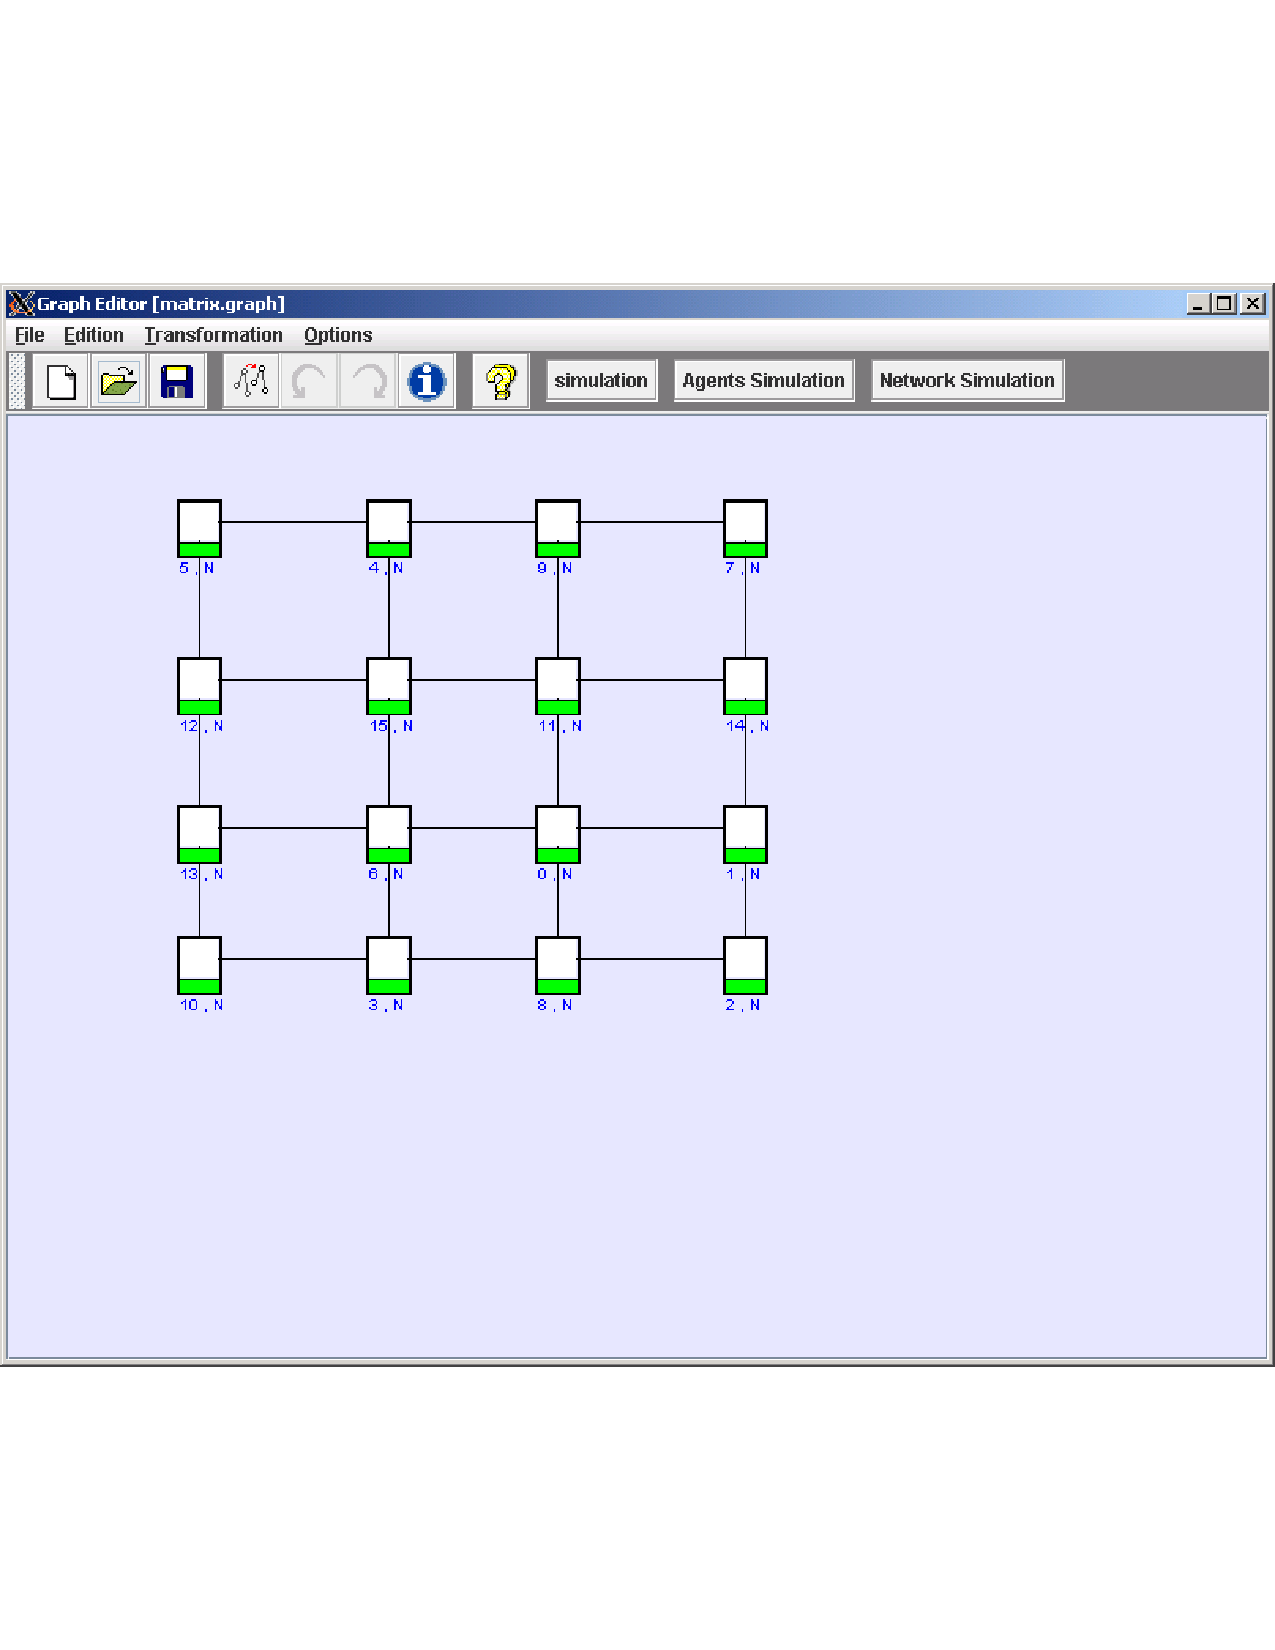
\includegraphics[width=10cm]{fonctionnement-matrix-graph}
  \caption{}
  \label{fig:fonctionnement-matrix-graph}
\end{figure}


2 ajout des agents

\begin{figure}[ht]
  \centering
  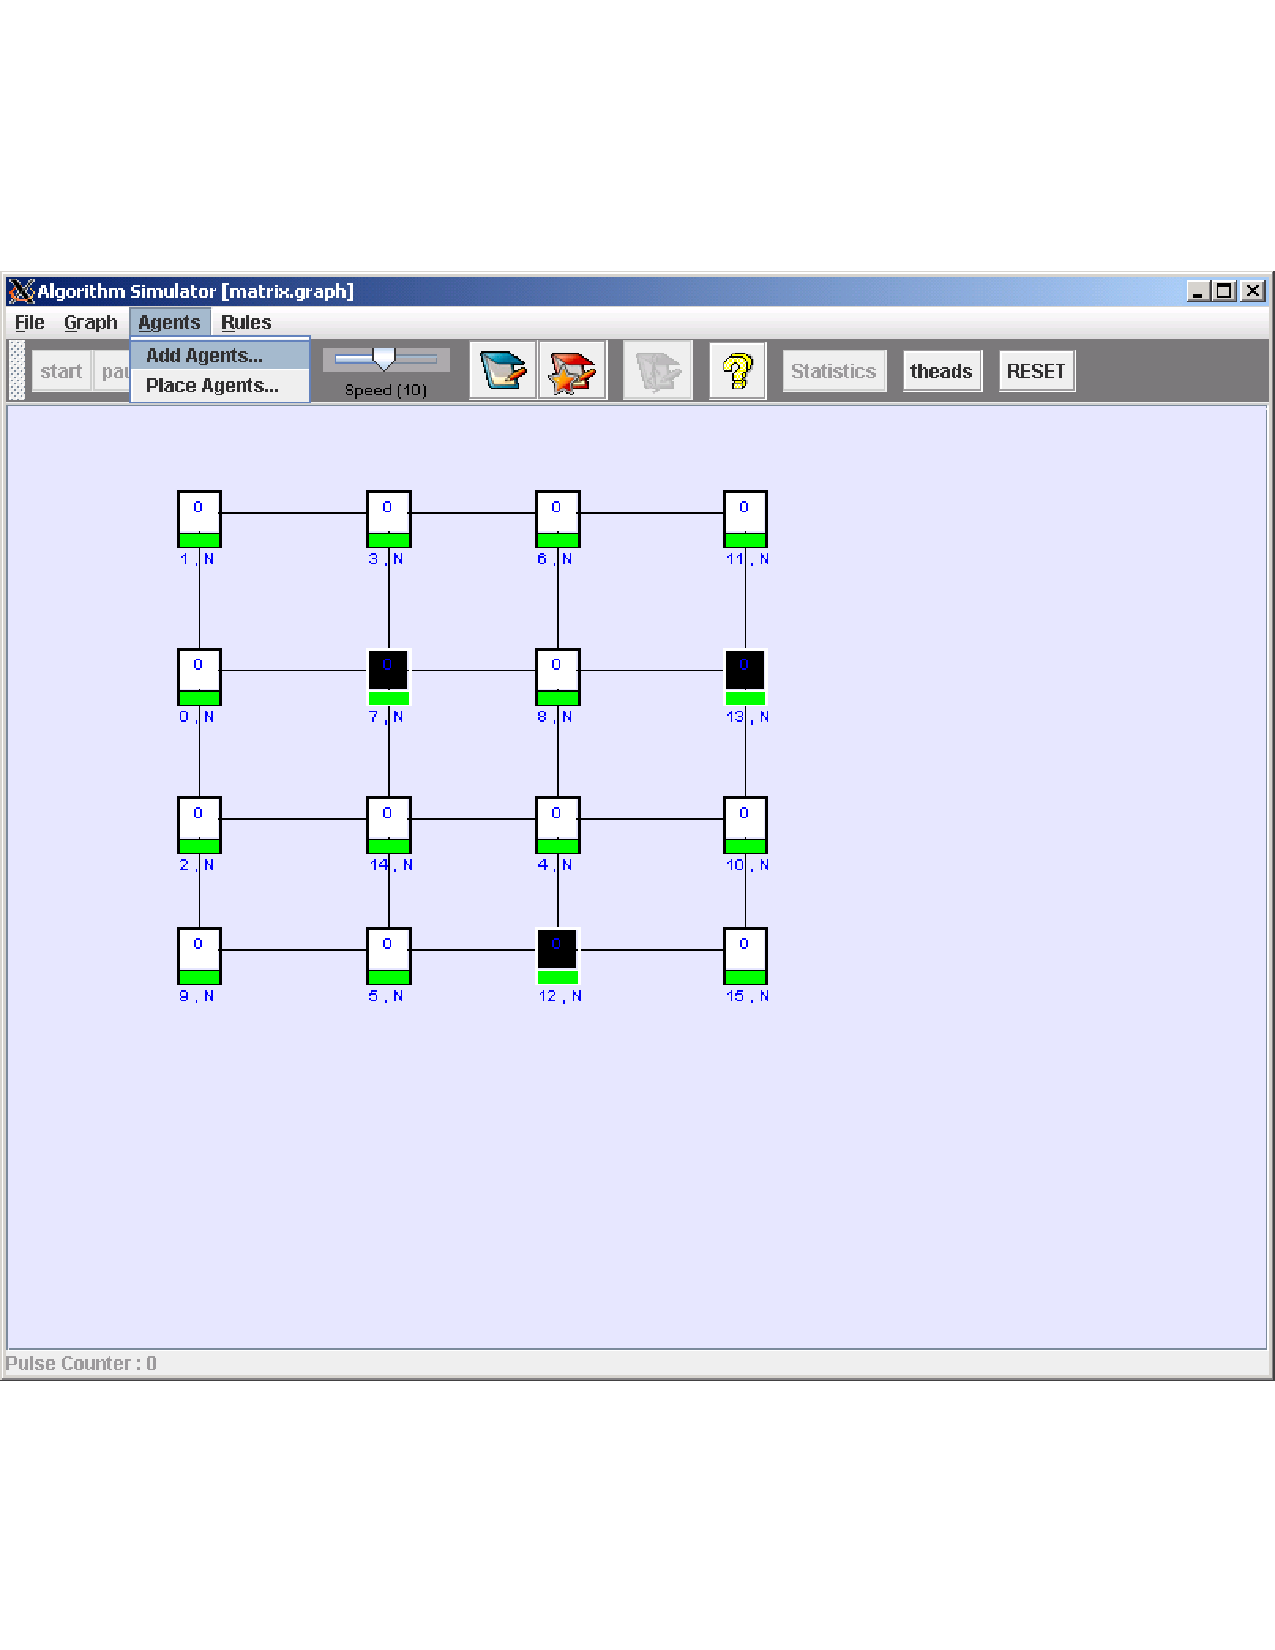
\includegraphics[width=10cm]{fonctionnement-ajout-agent}
  \caption{}
  \label{fig:fonctionnement-ajout-agent}
\end{figure}

3 choix des agents

\begin{figure}[ht]
  \centering
  \includegraphics[width=10cm]{fonctionnement-choix-agent}
  \caption{}
  \label{fig:fonctionnement-choix-agent}
\end{figure}

4 simulation en cours

\begin{figure}[ht]
  \centering
  \includegraphics[width=10cm]{fonctionnement-sumu1}
  \caption{}
  \label{fig:fonctionnement-simu1}
\end{figure}

5 visualisation whiteboard sommet

\begin{figure}[ht]
  \centering
  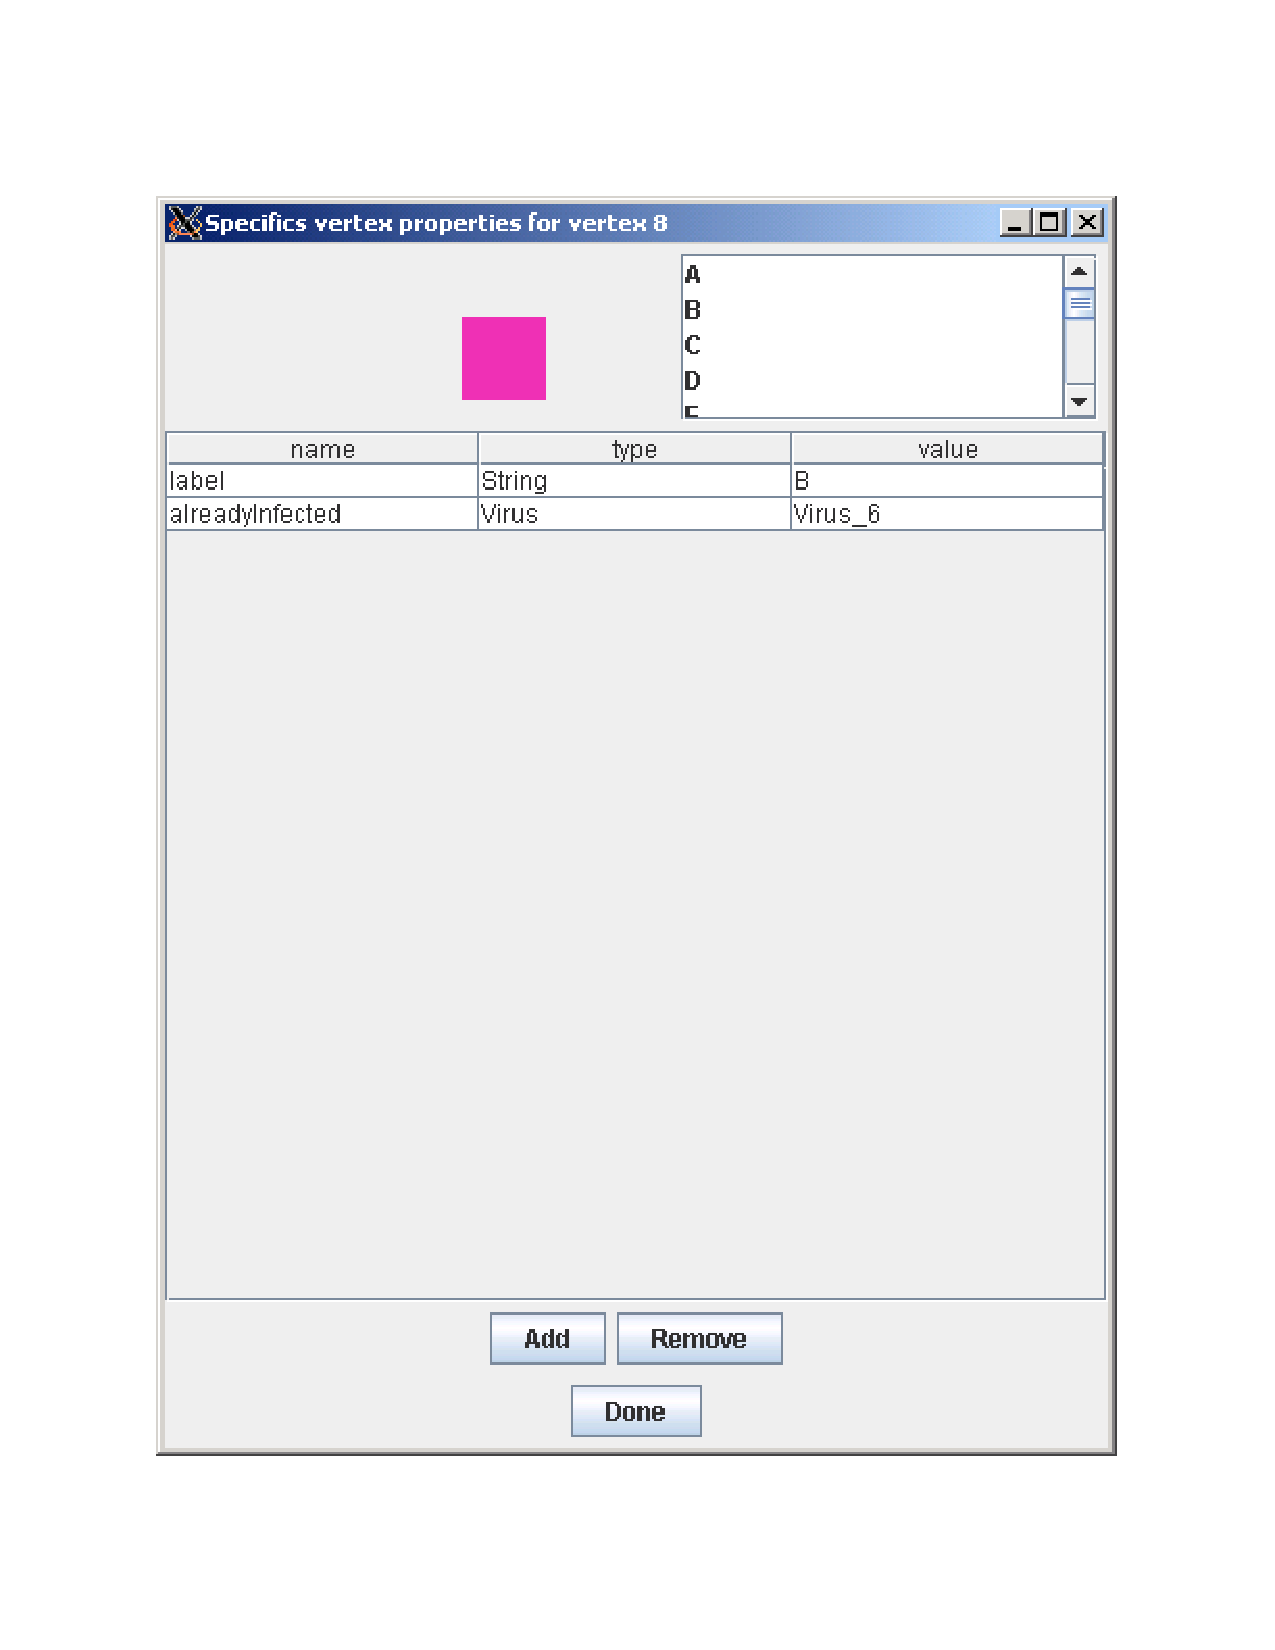
\includegraphics[width=10cm]{fonctionnement-vertex-properties}
  \caption{}
  \label{fig:fonctionnement-vertex-properties}
\end{figure}

6 simu-termin�

\begin{figure}[ht]
  \centering
  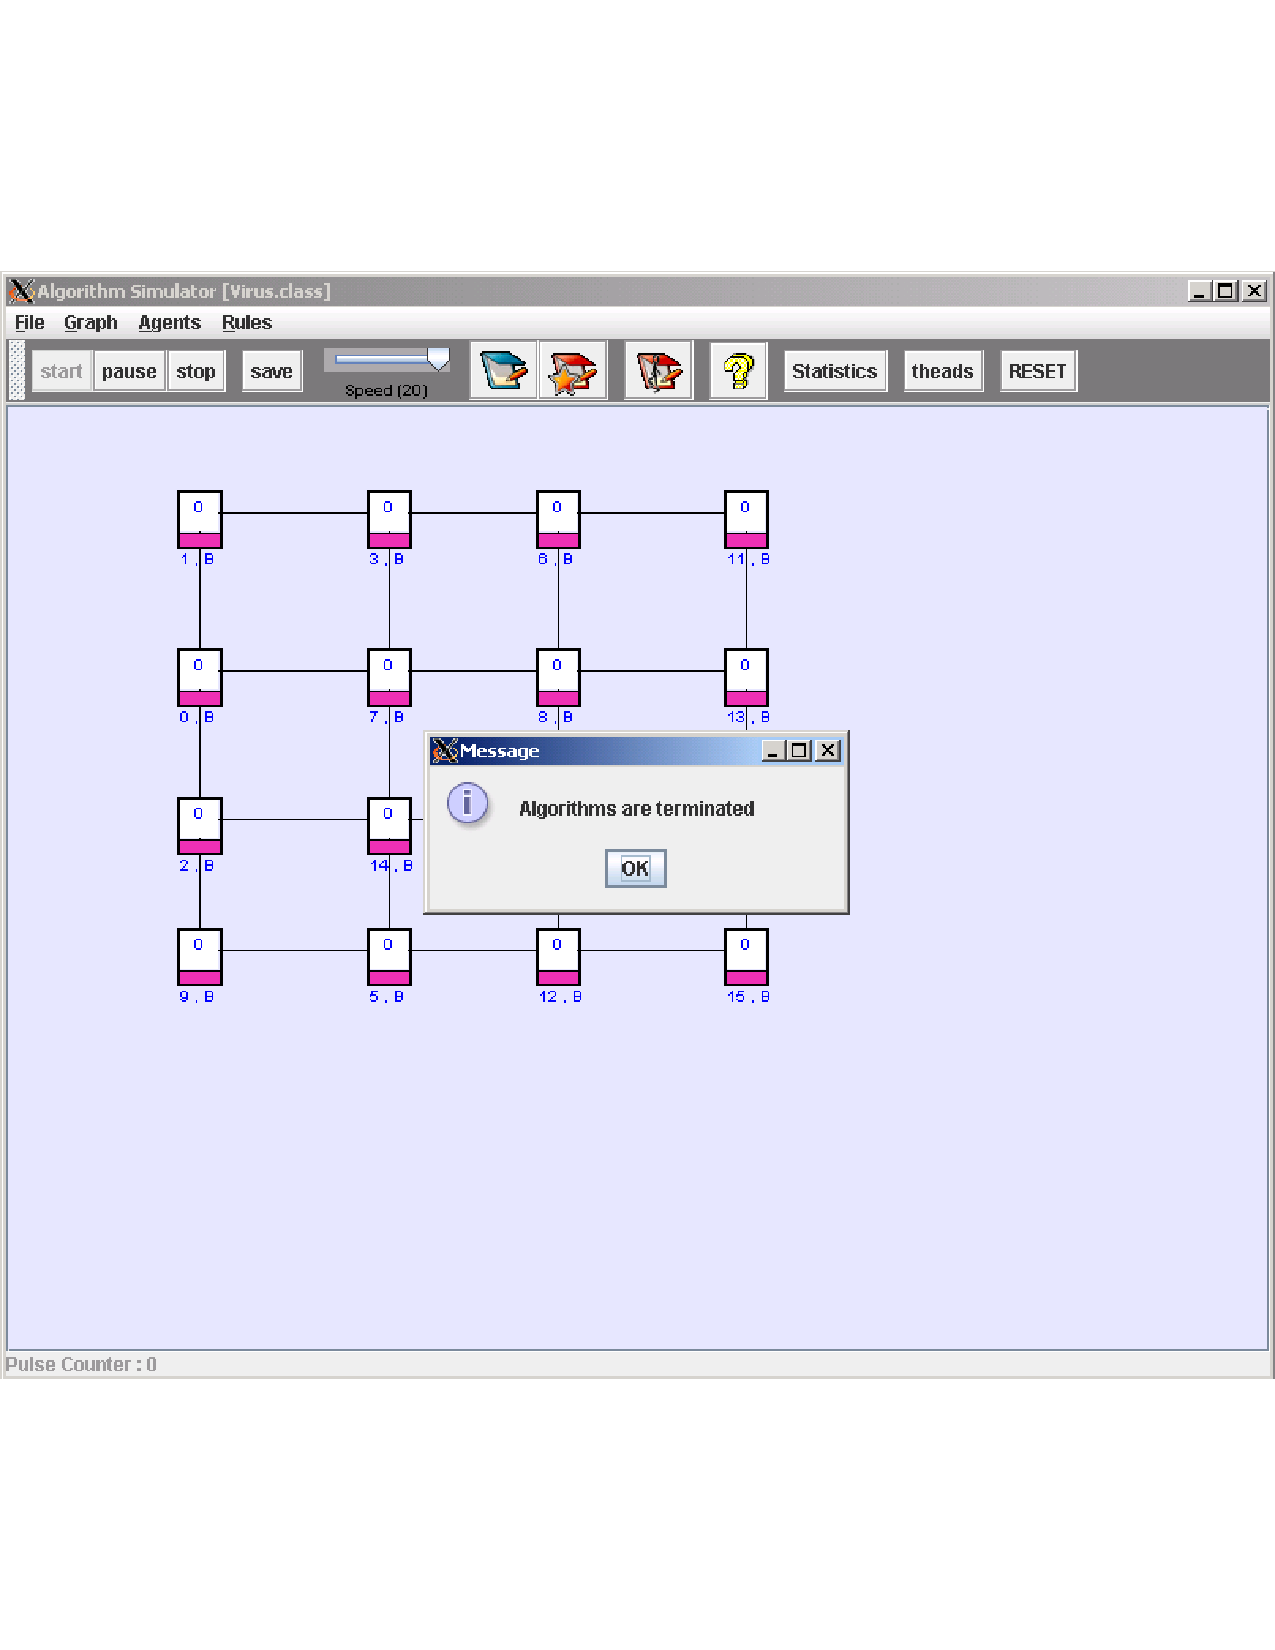
\includegraphics[width=10cm]{fonctionnement-simu-terminated}
  \caption{}
  \label{fig:fonctionnement-simu-terminated}
\end{figure}

7 choix stats

\begin{figure}[ht]
  \centering
  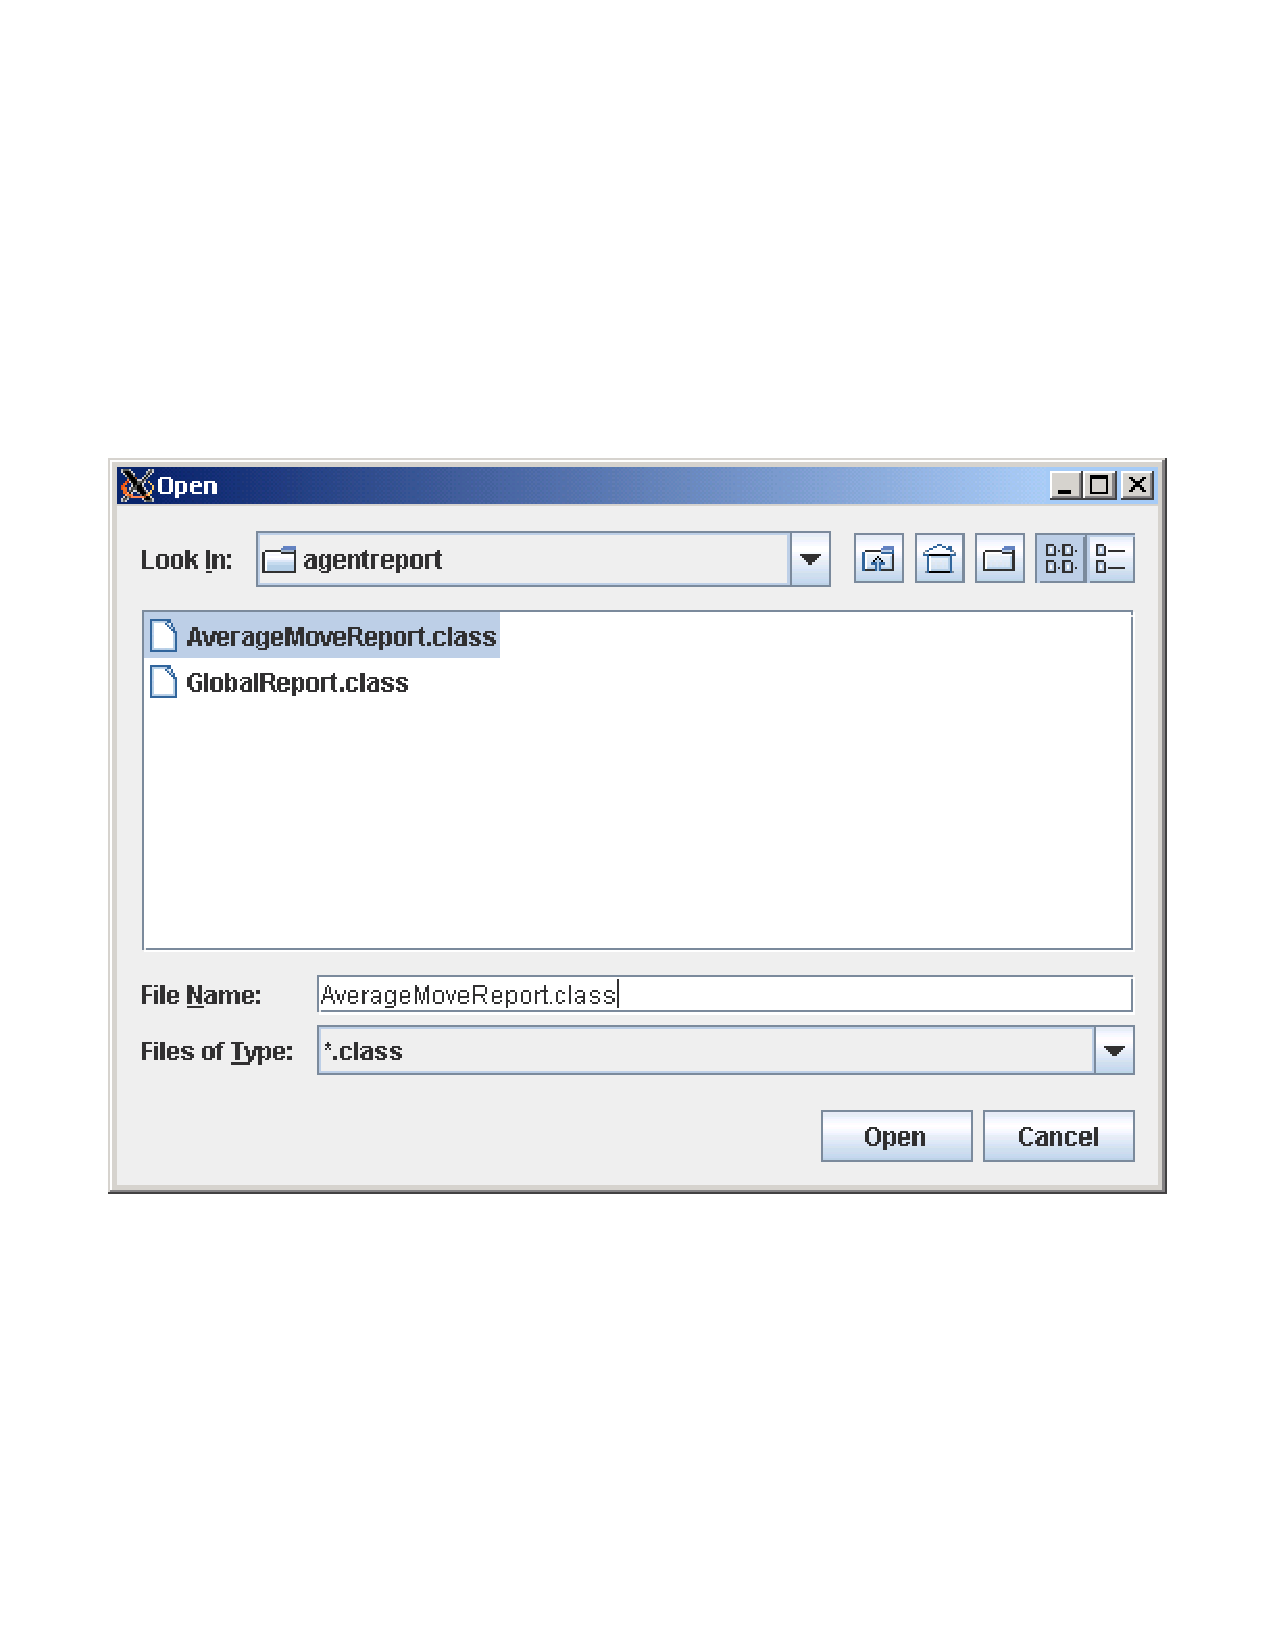
\includegraphics[width=10cm]{fonctionnement-choix-stats}
  \caption{}
  \label{fig:fonctionnement-choix-stats}
\end{figure}

8 resultats-stats

\begin{figure}[ht]
  \centering
  \includegraphics[width=10cm]{}
  \caption{}
  \label{fig:}
\end{figure}



\paragraph{Ecriture d'un algorithme}




%%% Local Variables: 
%%% mode: latex 
%%% TeX-master:  "rapport" 
%%% TeX-PDF-mode: t 
%%% coding:latin-1 
%%% End:
